\newif\ifsubmit
\submitfalse

\documentclass[acmsmall,review,anonymous]{acmart}%
\settopmatter{printfolios=true,printccs=false,printacmref=false}

% Encoding and lang
\usepackage[T1]{fontenc}
\usepackage[utf8]{inputenc}
\usepackage[english]{babel}

% Graphical packages
\usepackage{graphicx}

% Math
\usepackage{amsmath}
\usepackage{amsfonts}
\usepackage{amssymb}
\usepackage{amsthm}
% \usepackage{mathrsfs}
\usepackage{mathtools}
% \usepackage{textcomp}
% \usepackage{textgreek}
\usepackage{cmll}
\usepackage{mathpartir}

% Good citations and bibliography
\usepackage{natbib}

% % Pictures and latex lists
% \usepackage{wrapfig}
% \usepackage{float}
\usepackage{caption}
\usepackage{subcaption}
% \usepackage{placeins}
% \usepackage{array}
% \usepackage{paralist}
\usepackage{enumitem}% Compact lists
\usepackage{pifont}

% Specialized packages
% \usepackage{syntax} % Grammar definitions
\usepackage{verbatim}
\usepackage{listings} % Code
\usepackage{xspace} % Useful for macros
\usepackage{mathpartir}

\usepackage{textcomp}

\usepackage[noabbrev,nameinlink,capitalize]{cleveref}

% Custom macros

\newcommand{\ie}[0]{{i.e.}, }
\newcommand{\eg}[0]{{e.g.}, }

\newcommand\TODO[1]{{\ \\\color{red}\large\textbf{TODO} #1}\\}

\newcommand\mysc[1]{{\textsc{#1}}\xspace}
\newcommand\ocaml{\mysc{OCaml}}
\newcommand\haskell{\mysc{Haskell}}

\newcommand\htag[1]{\shortintertext{\textbf{#1}}}


\newcommand\code[2][]{\mbox{\lstinline[#1,basicstyle=\ttfamily\normalsize]{#2}}}

% Colors!
\definecolor{butter}{HTML}{C4A000}
\definecolor{orange}{HTML}{CE5C00}
\definecolor{chocolate}{HTML}{8F5902}
\definecolor{chameleon}{HTML}{4E9A06}
\definecolor{skyblue}{HTML}{204A87}
\definecolor{plum}{HTML}{5C3566}
\definecolor{scarletred}{HTML}{A40000}
\definecolor{lightalu}{HTML}{BABDB6}
\definecolor{darkalu}{HTML}{2E3436}
\newcommand{\kwstyle}{}

\lstdefinelanguage{Haskell}{
  otherkeywords={|,=>,<=,<,>,::,=,@,||,\$},%
  keywords=[1]{if,then,else,case,in,let,where,do},
  keywords=[2]{class,data,newtype,of,deriving,type,sig},%
  keywords=[3]{hiding,infix,infixl,infixr,import,instance,module,qualified},%
  keywordstyle=\kwstyle,
  keywordstyle=[1]\kwstyle\color{chameleon},
  keywordstyle=[2]\kwstyle\color{scarletred},
  keywordstyle=[3]\kwstyle\color{skyblue},
  keywordstyle=[4]\kwstyle\color{butter},
  keywordstyle=[5]\kwstyle\color{skyblue},
  keywordstyle=[6]\kwstyle\color{skyblue},
  keywordstyle=[7]\kwstyle\color{chameleon},
  keywordstyle=[8]\kwstyle\color{butter},
  keywordstyle=[9]\kwstyle\color{butter},
  sensitive,%
  comment=[l]{--},%
  comment=[n]{\{-}{-\}},%
  string=[b]",%
  literate={->}{{{\kwstyle\color{chameleon}->}}}2
}%

%% Code listing
\lstset{
  tabsize=4,
  aboveskip={0.5\baselineskip},
  belowcaptionskip=0.5\baselineskip,
  columns=fixed,
  showstringspaces=false,
  extendedchars=true,
  breaklines=true,
  frame=none,
  basicstyle=\small\ttfamily, %\scriptsize\ttfamily
  keywordstyle=\bfseries,
  commentstyle=\itshape\color{gray},
  % identifierstyle=\color{blue!80!black},
  stringstyle=\color{purple!40!black},
  numbersep=5pt,
  numberstyle=\tiny\color{gray},
  escapeinside={(*@}{@*)},
  numbers=left,
  emphstyle=\color{green!60!black}\bfseries,
  emphstyle={[2]\color{blue!60!black}\bfseries},
  language=Haskell
}




%%% regular expressions
\newcommand\Rnull{\mathbf0}
\newcommand\Rempty{\mathbf1}
\newcommand\Runion[1]{#1 +}
\newcommand\Rconcat[1]{#1 \cdot}
\newcommand\Rstar[1]{#1^*}
\newcommand\Rintersect[1]{#1 \with}
\newcommand\Rcomplement{\texttildelow}

%%% misc
\newcommand\ltext[1]{\makebox[0pt][r]{\text{#1}\quad}}
\newcommand\lleq{\le_{ll}}

%%% Local Variables:
%%% mode: latex
%%% TeX-master: "main"
%%% End:


% Declare a new environment for floating examples. Used like figure.
\usepackage{newfloat}
\DeclareFloatingEnvironment[
listname={List of Examples},
name={Example},
placement={!ht},
]{ex}
\crefname{ex}{Example}{Examples}
\Crefname{ex}{Example}{Examples}
\crefname{subex}{Example}{Examples}
\Crefname{subex}{Example}{Examples}

% Bibliography
\bibliographystyle{ACM-Reference-Format}
\citestyle{acmauthoryear}

%% Journal information
%% Supplied to authors by publisher for camera-ready submission;
%% use defaults for review submission.
\acmJournal{PACMPL}
\acmVolume{1}
\acmNumber{ICFP} % CONF = POPL or ICFP or OOPSLA
\acmArticle{1}
\acmYear{2018}
\acmMonth{1}
\acmDOI{} % \acmDOI{10.1145/nnnnnnn.nnnnnnn}
\startPage{1}


\begin{document}

\title{Regenerate: A Language Generator for Extended Regular Expressions}

\author{Gabriel Radanne}
\affiliation{
  \institution{University of Freiburg}
  \country{Germany}
}
\email{radanne@informatik.uni-freiburg.de}

\author{Alexander Thiemann}
\affiliation{
\institution{University of Freiburg}
\country{Germany}
}
\email{mail@athiemann.net}

\author{Peter Thiemann}
\affiliation{
  \institution{University of Freiburg}
  \country{Germany}
}
\email{thiemann@acm.org}

\begin{abstract}
  \TODO{}
\end{abstract}
\keywords{\TODO{}}

\maketitle
\section{Introduction}

\TODO{}

The implementation will be available on Github and will be submitted for artifact evaluation. 


We assume familiarity with Haskell throughout the paper.  Some
familiarity with formal languages is helpful, but not required as the
paper contains all relevant definitions. Our notation for formal
languages is borrowed from one of the classic textbooks on the topic
\cite{DBLP:books/daglib/0011126}.

%%% Local Variables:
%%% mode: latex
%%% TeX-master: "main"
%%% End:

\section{Motivation}
\label{sec:motivation}

Suppose someone implemented a clever algorithm for
regular expression matching. 
We want to use this implementation, but we also want to play safe and
make sure it is largely bug free by subjecting it to extensive
testing---verification is deemed to expensive.
Such testing requires us to come up with test cases and
implement a test oracle.


A test case consists of a regular expression \code{r} and an input
string \code{s}. If \code{match} is the implementation of matching
and \code{matchOracle} is the test oracle, then
executing the test case means to execute \code{match r
  s} and check whether the result is correct by comparing it with
\code{matchOracle r s}. 

A popular way of conducting such a test is using the QuickCheck library
\cite{quickcheck}, which performs property-based random testing. Using
QuickCheck, we would write a random generator for regular expressions
and then use the random generator for strings to generate many inputs for a
generated regular expression.

However, this approach has a
catch. Depending on the language of the regular expression, the
probability that a random string is a member of the language can be
severely skewed. As an example, consider the language $L = (ab)^*$ over the
alphabet $\Sigma = \{a, b\}$. Although $L$ contains infinitely many
words, the probability that a random word of
length $n$ is an element of $L$ is
\begin{itemize}
\item $0$ if $n$ is odd and
\item $\frac{1}{2^n}$ if $n$ is even.
\end{itemize}
Thus, the probability $p_n$ that a random word of length less than or equal to
$n$ is an element of $L$ is very small:
\begin{align*}
  p_n &= \frac{\lfloor n/2 \rfloor}{2^{n+1} - 1}
        \le \frac{n}{2^{n+2} - 2}
\end{align*}
Hence, the probability of (uniformly) randomly
selecting a word in $L$ is zero in the limit.

Hence, there are two problems with testing the regular expression
matcher.
\begin{enumerate}
\item How do we know whether the test oracle is correct, short of
  verifying it?
\item How do we ensure that relevant test cases are generated, given
  that the probability of randomly picking a word in the language is
  $0$ or $1$ for many regular languages?\footnote{Exercise for the
    interested reader:
    \begin{enumerate}
    \item Come up with a regular language $R$ such that $P(w\in R)$ is
      different from $0$ or $1$.
    \item Given a proper fraction $m/n$ (that is $n>0$ and $0\le m\le
      n$) define a regular language $R$ such that $P (w\in R) = m/n$.
    \end{enumerate}
  }
\end{enumerate}


Wouldn't it be nice to have a systematic and obviously correct means
of generating words \textbf{inside} of $L$ and \textbf{outside} of
$L$? Such a generation algorithm would obviate the need for an oracle
and it would make sure that we can control the number of test inputs
in the language and in the language's complement.

In the follwing we will tackle a slightly more general question, namely generating
the language of a \emph{generalized regular expression}, 
which subsumes the purpose of generating positive and negative sample
words for testing.

\subsection{Brief Intermezzo on Formal Languages}
\label{sec:research-question}

\begin{figure}[tp]
  \begin{align*}
    r, s & &L(\_)=\quad &  &
                             \makebox[1em][l]{\code{data GRE sig}}\\
         & ::= \Rnull & \ltext{empty}
                        & \emptyset
                           &&\code{= Zero}\\
         & \mid \Rempty & \ltext{empty word}
                        & \{ \varepsilon \}
                           && \code{| One}\\
         & \mid (a \in \Sigma) & \ltext{singleton}
                        &  \{ a \}
                           && \code{| Atom sig} \\
         & \mid \Runion rs & \ltext{alternative}
                        &  L (r) \cup L (s)
                           && \code{| Or (GRE sig) (GRE sig)}\\
         & \mid \Rconcat rs & \ltext{concatenation}
                        &  L (r) \cdot L (s)
                           && \code{| Dot (GRE sig) (GRE sig)}\\
         & \mid \Rstar r & \ltext{Kleene star}
                        & (L (r))^* 
                           && \code{| Star (GRE sig)}\\
         & \mid \Rintersect rs & \ltext{intersection}
                        & L (r) \cap L (s)
                           && \code{| And (GRE sig) (GRE sig)}\\
         & \mid \Rcomplement r & \ltext{complement}
                        & \Sigma^* \setminus L (r)
                           && \code{| Not (GRE sig)}
  \end{align*}
  % \begin{align*}
  %   L (\Rnull) &= \emptyset\\
  %   L (\Rempty) &= \{ \varepsilon \} \\
  %   L (a) &= \{ a \} \\
  %   L (\Runion rs) &= L (r) \cup L (s) \\
  %   L (\Rconcat rs) &= L (r) \cdot L (s) \\
  %   L (\Rstar r) &= (L (r))^* \\
  %   L (\Rintersect rs) &= L (r) \cap L (s) \\
  %   L (\Rcomplement r) &= \Sigma^* \setminus L (r)
  % \end{align*}
  \caption{Generalized regular expressions}
  \label{fig:generalized-regular-expressions}
\end{figure}

As customary, we write $\Sigma^*$ for the set of finite words over
alphabet $\Sigma$, which is defined inductively as the smallest set
such that $\varepsilon \in
\Sigma^*$ and $\forall a\in\Sigma, \forall w\in\Sigma^*, aw \in \Sigma^*$.
The semantics of an expression, $L(r) \subseteq \Sigma^*$, is a set of
words, which is also defined in
Figure~\ref{fig:generalized-regular-expressions}. It relies on
standard definitions from the theory of formal languages. We write
$\varepsilon$ for the empty word and $u\cdot v$ for the concatenation
of words $u, v \in \Sigma^*$. We write $|u|$ for the length of word
$u$. Unless otherwise specified, we use $a, b, c, \dots$ to range over
$\Sigma$ and $u, v, w, \dots$ to range over $\Sigma^*$.

If $U, V \subseteq \Sigma^*$ are
languages, then their concatenation (or product) is defined as $U\cdot
V = \{ u\cdot v \mid u\in U, v\in V\}$. We sometimes write $u\cdot V$
as an abbreviation for the product $\{u\}\cdot V$ with a singleton
language. The Kleene closure of a
language $U\subseteq \Sigma^*$ is defined as $U^* =
\bigcup_{i=0}^\infty U^i$ where $U^0 = \{\varepsilon\}$ and $U^{i+i} =
U \cdot U^i$. 

A generalized regular expression
(Figure~\ref{fig:generalized-regular-expressions}) is an expression
built from the regular operators empty set, empty word, singleton word
consisting of a single letter $a$ chosen from a finite alphabet
$\Sigma$, alternative, concatenation, and Kleene star. In addition, it
may contain the operators intersection and complement. The extra
operators do not add extra descriptive power as regular languages are
closed under intersection and complement \cite{AhoHopcroftUllman}, but
generalized regular expressions can be much more concise. 



\subsection{Naive Approach}
\label{sec:naive-approach}

We start with a naive implementation of the mathematical definition in
Figure~\ref{fig:generalized-regular-expressions}. We define an
alphabet by a list of \code{Char}.  We represent words by elements of Haskell's
\code{Data.Text.Text} datatype, abbreviated to \code{T.Text}. We
represent a language as a lazy list of \code{Text}, as a language
can be an infinite set. There are two further restrictions.
\begin{enumerate}
\item The output of a generator should not contain repetitions
  because we would like to guarantee that test inputs are different
  from each others.
\item The output of a generator should not be partial because it would
  lead the test code to hang on a nonterminating input.
\end{enumerate}

\begin{lstlisting}
import Data.Text as T

type Alphabet = [Char]
type Lang = [T.Text]

generate :: Alphabet -> GRE Char -> Lang
generate sigma r = gen r
  where
    gen Zero = []
    gen One  = [T.empty]
    gen (Atom t) = [T.singleton t]
    gen (Or r s) = union (gen r) (gen s)
    gen (Dot r s) = concatenate (gen r) (gen s)
    gen (Star r) = star (gen r)
    gen (And r s) = intersect (gen r) (gen s)
    gen (Not r) = complement sigma (gen r)
\end{lstlisting}
\begin{figure}[tp]
\begin{lstlisting}
module Examples.Naive where
import qualified Data.Text as T

union :: Lang -> Lang -> Lang
union lx ly = lx ++ ly

concatenate :: Lang -> Lang -> Lang
concatenate lx ly = [T.append wx wy | wx <- lx, wy <- ly ]

intersect :: Lang -> Lang -> Lang
intersect lx ly = [wx | wx <- lx, wx `elem` ly ]

star :: Lang -> Lang
star lx = concat lxi
  where
    lxi = [T.empty] : map (concatenate lx) lxi

complement :: Alphabet -> Lang -> Lang
complement sigma lx =
  undefined
\end{lstlisting}
  \caption{Partial implementation of the regular operators}
  \label{fig:regular-operators-0}
\end{figure}
As a basis for further discussion, we exhibit a partial 
implementation in Figure~\ref{fig:regular-operators-0}.
This implementation has a number of deficiencies.
\begin{description}
\item[union] The output may contain duplicates. If
  \texttt{lx} is infinite, then no words from \texttt{ly} will ever be
  produced. This behavior violates the specification of set union
  because there may be elements in \texttt{ly} that never appear in
  \texttt{union lx ly}.

  If we restricted ourselves to finite lists, then replacing
  \texttt{++} with \texttt{Data.List.union} would be an appropriate
  implementation, but its worst-case time complexity is quadratic.
\item[concatenate] The output may contain duplicates. If \texttt{ly}
  is infinite, then only the first word in \texttt{lx} contributes to
  the output.

  For finite lists, an appropriate implementation would compose the
  raw product computation with \texttt{Data.List.nub} to remove
  duplicates. The worst-case complexity of \texttt{nub} is quadratic.
\item[intersect] The output contains no duplicates, if \texttt{lx}
  does not contain duplicates, either. If \texttt{ly} is infinite,
  then the resulting list may be partial because the \texttt{elem}
  operation may not terminate.

  For finite lists, this implementation is appropriate.
\item[star] The output may contain duplicates. If \texttt{lx} is
  infinite, then the generated language is just \texttt{T.empty : lx},
  so that many elements of \texttt{star lx} may not appear in the
  output.

  If \texttt{lx} is finite, then \texttt{star} can
  be implemented in a way that guarantees no duplication. However, to
  retain finiteness, we would have to impose an arbitrary limit on the
  size of the output.
\item[complement] In general there is no computable way to determine
  whether a word occurs in a lazy list \texttt{lx}. Hence, we have no
  good definition to propose.

  If \texttt{lx} is finite, then it is possible to
  enumerate its complement without repetitions. Again, to retain
  finiteness, we have to impose an arbitrary limit on the size
  of the output.
\end{description}
\begin{figure}[tp]
\begin{lstlisting}
module Examples.Finite where
import qualified Data.Text as T
import Data.List as L

limit :: Int
limit = 1024

union :: Lang -> Lang -> Lang
union lx ly = L.union lx ly

concatenate :: Lang -> Lang -> Lang
concatenate lx ly = L.nub [T.append wx wy | wx <- lx, wy <- ly ]

intersect :: Lang -> Lang -> Lang
intersect lx ly = [wx | wx <- lx, wx `elem` ly ]

star :: Lang -> Lang
star lx = take limit $ removeDuplicates $ concat lxs
  where
    lxs = [T.empty] : map (concatenate lx1) lxs
    lx1 = L.delete T.empty lx
    removeDuplicates [] = []
    removeDuplicates (w:ws) = w : removeDuplicates (filter (/=w) ws)

complement :: Alphabet -> Lang -> Lang
complement sigma lx = take limit (concat lsigmastar L.\\ lx) 
  where
    lsigmastar =
      [T.empty] : 
      map (\lsigmai -> concatMap (\la -> concatenate la lsigmai) lsigma1) lsigmastar
    lsigma1 = map (return . T.singleton) sigma
\end{lstlisting}
  \caption{Finite implementation of the regular operators}
  \label{fig:finite-regular-operators}
\end{figure}
Figure~\ref{fig:finite-regular-operators} contains an implementation
of a finite version of the generator module according to the preceding
discussion. The implementation of \texttt{star} follows the definition
of $U^*$ literally. It first recursively creates a list \texttt{lxs}
of the iterates $U_\bullet^i$ where
$U_\bullet = U \setminus \{\varepsilon\}$, concatenates all of
them\footnote{It is easy to see that $U^* = U_\bullet^*$.}, removes
the duplicates, and imposes the limit. Removing duplicates introduces
quadratic worst-case time complexity in the size of the output.

The implementation of \texttt{complement} generates the language
$\Sigma^*$ analogously to the construction of $U^*$ in
\texttt{star}, uses the list difference operator
\texttt{L.\textbackslash\textbackslash} to remove elements of
\texttt{lx}, and finally imposes the limit. Its worst-case run time is
$O(m\cdot n)$ where $m$ is the limit and $n = \code{length lx}$.

In summary, the naive approach in
Figure~\ref{fig:regular-operators-0} can generate infinite languages,
but has many drawbacks that lead to duplication and incompleteness
(words in the language are not enumerated). Moreover, the complement
is not computable for this approach.

The finite approach in Figure~\ref{fig:finite-regular-operators}
imposes an arbitrary limit on the number of generated words. This
limit can lead to omitting words in nonempty languages where $P (w\in
R) = 0$. Moreover, there are many places (in \texttt{union},
\texttt{concatenate}, and \texttt{star}) with quadratic worst-case
time complexity. 

At this point, the question is: Can we do better? Can we come up with
a generator that supports finite as well as infinite languages
efficiently without incurring extraneous quadratic behavior?


\subsection{Ordered Enumeration}
\label{sec:ordered-enumeration}
\begin{figure}[tp]
\begin{lstlisting}
union :: (Ord t) => [t] -> [t] -> [t]
union xs@(x:xs') ys@(y:ys') =
  case compare x y of
    EQ -> x : union xs' ys'
    LT -> x : union xs' ys
    GT -> y : union xs ys'
union xs ys = xs ++ ys
\end{lstlisting}

\begin{lstlisting}
intersect :: (Ord t) => [t] -> [t] -> [t]
intersect xs@(x:xs') ys@(y:ys') =
  case compare x y of
    EQ -> x : intersect xs' ys'
    LT -> intersect xs' ys
    GT -> intersect xs ys'
intersect xs ys = []
\end{lstlisting}

\begin{lstlisting}
difference :: (Ord t) => [t] -> [t] -> [t]
difference xs@(x:xs') ys@(y:ys') =
  case compare x y of
    EQ -> difference xs' ys'
    LT -> x : difference xs' ys
    GT -> difference xs ys'
difference xs ys = xs
\end{lstlisting}
  \caption{Union, intersection, and difference by merging lists}
  \label{fig:merging-lists}
\end{figure}

First, we concentrate on improving on the quadratic behavior. The key
to improve the complexity of union, intersection, and complement lies
in representing a language by a strictly increasingly sorted list.
In this case, the three operations can be implemented by variations of
the merge operation on lists as shown in
Figure~\ref{fig:merging-lists}.

The merge-based operations run in linear time on finite
lists. However, the operations in Figure~\ref{fig:merging-lists} are
incomplete on infinite lists. As 
an example of the incompleteness, consider the languages $U = a\cdot
(a+b)^*$ and the singleton language $V = \{b\}$ where $\Sigma = \{a, b\}$
with $a<b$, represented as strictly increasing lists, the infinite
list \code{lu} and the singleton list \code{lv}. The problem is that
the list \code{union lu lv} does not contain the word $b$; more
precisely, \code{T.singleton 'b' `elem` union lu lv} does not
terminate whereas \code{u `elem` union lu lv} yields \code{True} for
all \code{u} in \code{lu}. The source 
of the problem is that Haskell's standard ordering of lists and
\code{Text} is the \emph{lexicographic ordering}, which we call
$\le$. It relies on an underlying total ordering on $\Sigma$ and is
defined inductively:
\begin{mathpar}
  \inferrule{}{\varepsilon  \le v}
  
  \inferrule{u \le v}{au \le av}

  \inferrule{a < b}{au \le bv}
\end{mathpar}

This total ordering
is often used for $\Sigma^*$, but it has the property that
there are words $v<w$ such that there are infinitely many words $u$
with $v<u$ and $u<w$. For example, $v=a$, $w=b$, and $u\in U \setminus
\{a\}$, which explains the nonterminating behavior just exhibited.

Fortunately, there is another total ordering on words with better
properties. The
\emph{length-lexicographic ordering} is defined by $u \lleq 
v$ if $|u|<|v|$ or $|u|=|v|$ and $u\le v$ in the usual lexicographic
ordering (but only applied to words of the same length). Here is a definition in Haskell.
\begin{lstlisting}
llocompare :: T.Text -> T.Text -> Ordering
llocompare u v =
  case compare (T.length xs) (T.length ys) of
    EQ -> compare xs ys
    LT -> LT
    GT -> GT
\end{lstlisting}
This ordering has the additional advantage that it gives raise to a standard
enumeration of all words over a totally ordered alphabet as an order-preserving
bijective function from the natural numbers to $\Sigma^*$. Using this
bijection we can show that for each pair of words $v \lleq w$ there is only a finite
number of words $u$ such that $v \lleq u$ and $u \lleq w$. 

For the sake of simplicity, we assume from now on that \code{T.Text}
is ordered by \code{llocompare} and call the representation of a
language by a strictly increasing list in length-lexicographic order
its \emph{LLO representation}. 

With the LLO representation, the operations \code{union},
\code{intersect}, and \code{difference} run in linear time. If the input languages
are finite of size $m$ and $n$, respectively, then $O(m+n)$
comparisons, pattern matches, and cons operations are needed.
Moreover, the operations are complete in the sense that any element in
the output is sure to be detected by a terminating computation. 
It is easy to implement a version of \code{elem} that exploits the LLO ordering,
such that the element test is decidable for any infinite
language.



\subsubsection{Concatenation}
To implement concatenation, we are in the following situation. Given
two languages $U, V \subseteq \Sigma^*$ in LLO representation,
produce the LLO representation of $U \cdot V =  \{ u\cdot v \mid u\in
U, v\in V\}$. If we compute the product naively as in
Figure~\ref{fig:regular-operators-0}, then the output is not in LLO
form:\footnote{The example uses \code{String} for simplicity.}
\begin{verbatim}
λ> let lu = ["a", "ab"]
λ> let lv = ["", "b", "bb"]
λ> [ u++v | u <- lu, v <- lv ]
["a","ab","abb","ab","abb","abbb"]
\end{verbatim}
In fact, the output violates both constraints: it is not increasing
and it has duplicates.

Perhaps the following observation helps: for each $u\in U$, the LLO
representation of the language $u\cdot V$ can be trivially produced
because the list \code{[ u++v | v <- lv ]} is strictly
increasing. This observation motivates the following definition of
language concatenation (using \code{union} from Figure~\ref{fig:merging-lists}).
\begin{lstlisting}
concatenate' :: Lang -> Lang -> Lang
concatenate' lx ly =
  foldr union [] $ [[ T.append x y | y <- ly] | x <- lx]
\end{lstlisting}
This definition works fine as long as \code{lx} is finite. If it is
infinite, then the \code{foldr} creates an infinitely deep nest of
invocations of \code{union}, which do not make progress because
\code{union} is strict in both arguments.

At this point, the theory of formal languages can help. The notion of
a \emph{formal power series} has been invented to reason about and
compute with entire languages \cite{formal power series}. In full
generality, a formal power series is a mapping from $\Sigma^*$ into a
semiring $S$ and we write $\FPS{S}$ for the set of these
mappings. Formally, an element $r \in \FPS{S}$ is written as the
formal sum
\begin{align*}
  r &= \sum_{w \in \Sigma^*} (r,w) \cdot w
\end{align*}
where $(r,w) \in S$ is the coefficient of $w$ in $r$.
A popular candidate for this semiring is the boolean semiring $B$
because $\FPS{B}$ is isomorphic to the set of languages over
$\Sigma$. This isomorphism maps $L\subseteq\Sigma^*$ to its
characteristic series $r_L$ where $(r_L, w) = (w \in L)$.

The usual language operations have their counterparts on formal power
series. We consider just three of them where the ``additions'' and ``multiplications'' on the
right side of the definitions take place in the underlying semiring.
\begin{itemize}
\item Sum: $(r_1 + r_2, w) = (r_1, w) + (r_2, w)$ 
\item Product: $(r_1 \cdot r_2, w) = \sum_{uv=w} (r_1, u) (r_2,v)$
\item Hadamard product: $(r_1 \odot r_2, w) = (r_1, w) (r_2, w)$
\end{itemize}


\clearpage{}
%%% Local Variables:
%%% mode: latex
%%% TeX-master: "main"
%%% End:

\section{Improvements}
\label{sec:improvements}

\subsection{Segmented representation}
\label{sec:segm-repr}

Two operations on the LLO representation, \code{concatenate} and
\code{star}, internally transform their inputs into segment
sequences. Such a transformation forth an back seems wasteful, so we
stipulate to perform the entire generation in terms of segment
sequences. The transformation to a language only happens as the final
step.

As a second refinement, we try to address the productivity concern
discussed in Section~\ref{sec:motivation-discussion}. The approach is
to let finite segment sequences represent finite languages. Hence,
\begin{lstlisting}
  zero = []
  one = [[T.empty]]
  atom t = [[], [T.singleton t]]
\end{lstlisting}

We discuss the remaining issues with the code for concatenation.
\begin{lstlisting}
  concatenate lx ly = collect 0
    where
      collect n =
        (foldr ILO.union [] $ map (combine n) [0 .. n]) : collect (n+1)
      combine n i =
        [T.append x y | x <- lx !!! i, y <- ly !!! (n - i)]
\end{lstlisting}
The code relies on a special indexing operation that returns an empty
list if indexing occurs beyond the end of a segment list:
\begin{lstlisting}
(!!!) :: [[a]] -> Int -> [a]
[]       !!! n = []
(xs:xss) !!! 0 = xs
(xs:xss) !!! n = xss !!! (n - 1)
\end{lstlisting}
But the concatenation of finite languages still yields a partial list.

\clearpage{}
%%% Local Variables:
%%% mode: latex
%%% TeX-master: "main"
%%% End:

\section{\ocaml Implementation}
\label{sec:ocaml}

\lstset{language=[Objective]Caml}

We also implemented our
language generation algorithm in \ocaml.
% The \ocaml version only implements the ``latest'' version of the
% algorithm with a segmented representation, fast backward lookup and convolutions
% for concatenation and star, and symbolic representation of segments.
% One of the goal of this implementation was to test
% pure \ocaml regular expression libraries such as ocaml-re\footnote{\url{https://github.com/ocaml/ocaml-re}} and
% mulet\footnote{\url{https://github.com/let-def/mulet}}. 
The main goal of this implementation is to experiment with strictness
and various data structures for segments. 
The key idea is that the internal order on words in a segment does not matter
because each segment only contains words of the same length.
All we need is a data structure that supports the power series
operations.
%
To facilitate such experimentation, we implemented the
algorithm as a functor whose signature is shown in
\cref{code:sigs:segment,code:sigs:word,code:sigs:regen}.
\ocaml{} functors are parameterized modules that take modules
as argument and return modules. Our implementation
takes two data structures as arguments, words and segments,
to test different representations without changing
the code.
% It also forced us to find the minimal set of operations
% needed to implement the algorithm.

\begin{figure}[tp]
\begin{lstlisting}
module type WORD = sig
  type char
  type t
  val empty : t
  val singleton : char -> t
  val append : t -> t -> t
end
\end{lstlisting}
\vspace{-\baselineskip}
    \caption{Operations on words}
    \label{code:sigs:word}

\begin{lstlisting}
module type SEGMENT = sig
  type elt (* Elements *)
  type t (* Segments *)

  val empty: t
  val is_empty: t -> bool
  val singleton: elt -> t

  (* Set operations *)
  val union: t -> t -> t
  val inter: t -> t -> t
  val diff: t -> t -> t
  val append: t -> t -> t
  val merge: t list -> t

  (* Import/Export *)
  val of_list: elt list -> t
  val iter: t -> (elt -> unit) -> unit

  (** For transient data-structures *)
  val memoize: t -> t
end
\end{lstlisting}
\vspace{-\baselineskip}
    \caption{Operations on segments}
    \label{code:sigs:segment}
    
\begin{lstlisting}
module Regenerate
    (Word : WORD)
    (Segment : Segments.S with type elt = Word.t)
: sig
  type lang
  val gen : Segment.t -> Word.char regex -> lang
  val iter : lang -> (Word.t -> unit) -> unit
end
\end{lstlisting}
\vspace{-\baselineskip}
    \caption{Language generation as a functor}
    \label{code:sigs:regen}
\end{figure}

\paragraph{Characters and Words}

\autoref{code:sigs:word} contains the signature for words.
It provides
the empty word (for \code{One}),
singleton words (for \code{Atom}), and append.
Neither an ordering nor a length operation is needed:
Comparison is encapsulated in the segment
data structure and the length of a word is the index of the segment in
which it appears.
%
This signature is satisfied by the \ocaml \code{string}
type (\ie arrays of bytes), arrays, lists of characters, or ropes. The
type of individual characters is unrestricted.

\paragraph{Segments}

\autoref{code:sigs:segment} contains the signature for segments.
% The first group of operations creates and tests for empty segments and
% singleton segments. 
The main requirement is to support the operations on power series as described in \autoref{sec:gener-cross-sect} and the set operations
\code{union}, \code{inter} and \code{inter}.
%
The product described in \autoref{eq:1} is decomposed in two parts:
\begin{itemize}[leftmargin=*]
\item An \code{append} function to implement $U_i V_{n-i}$. It computes the
  product of two segments by appending their elements.
\item A \code{merge} operation which computes the union of an arbitrary number
  of segments. It collects the segments obtained
  by invocations of \code{append}.
\end{itemize}
%
Experimentation with transient data-structures requires
an explicit \code{memoize} function that avoids recomputing segments accessed
multiple times. 
%
Finally, the functions  \code{of_list} and \code{iter} import and
export elements to and from a segment.

\subsection{Core Algorithm}

The core algorithm follows the Haskell version. The power series
is implemented using a thunk list in the style of \citet{DBLP:conf/cpp/Pottier17}
with some special-purpose additions:

\begin{lstlisting}
type node =
  | Nothing
  | Everything
  | Cons of Segment.t * lang
and lang = unit -> node
\end{lstlisting}

An enumeration is represented by a function which takes a unit argument and returns
a node. A node, in turn, is either \code{Nothing} or a \code{Cons} of an
element and the tail of the sequence.
% The empty enumeration, for instance, is
% represented as \code{fun () -> Nothing}.
% This representation is lazy, fast, lightweight, and almost as easy to
% manipulate as regular lists.
% \footnote{See
%   \url{https://github.com/ocaml/ocaml/pull/1002} for a long discussion
%   on the topic.}
The additional constructor \code{Everything} allow to manipulate
full languages symbolically, as in \cref{sec:more-finite-repr}.

% The rest of the implementation is similar to the \haskell one.
As an example, the implementation of language union is shown below.
The trailing unit argument \code{()} drive the evaluation of the
sequence lazily. With this definition, \code{union s1 s2} cause no
evaluation before it is applied to \code{()}.
\begin{lstlisting}
let rec union s1 s2 () = match s1(), s2() with
  | Nothing, x | x, Nothing -> x
  | Everything, _ | _, Everything -> Everything
  | Cons (x1, next1), Cons (x2, next2) -> 
    Cons (Segment.union x1 x2, union next1 next2)
\end{lstlisting}

% The concatenation of languages demonstrates how the main algorithm can
% be expressed once the segment operations have been abstracted:.
% To build $U \cdot V$, we first build the $n$th term
% $(U \cdot V)_n = \bigcup_{i=0}^n U_i V_{n-i}$.
% We use both \code{Segment.append} to implement the product
% of segments and the concatenation of words and \code{Segment.merge} to merge
% all the resulting segments.
% \begin{lstlisting}
% let term_of_length map1 map2 n =
%   let combine_segments i =
%     Segment.append (IntMap.find i map1) (IntMap.find (n - i) map2)
%   in
%   List.(range 0 n) |> List.rev_map combine_segments |> Segment.merge
% \end{lstlisting}

% We then collect all the terms by synchronized recursion over the power series $U$
% and $V$:
% \begin{lstlisting}
% let rec collect n map1 map2 seq1 seq2 () = match seq1 (), seq2 () with
%   | Cons (segm1, seq1), Cons (segm2, seq2) ->
%     let map1 = IntMap.add n (Segment.memoize segm1) map1 in 
%     let map2 = IntMap.add n (Segment.memoize segm2) map2 in
%     Cons (term_of_length map1 map2 n, collect (n+1) map1 map2 seq1 seq2)
% \end{lstlisting}

% The \code{IntMap} module provides a functional implementation of maps
% keyed by integers. The maps are used to quickly access
% segments of smaller index that have been computed in earlier invocations of
% \code{collect}. As such segments are accessed
% multiple times, we use \code{memoize} to avoid computing them over and
% over again.
% Functional maps are sufficient because the size of a map is equal
% to the maximum word length, which does not get excessively large.

% Finally, we initialize \code{collect} with empty maps.
% \begin{lstlisting}[numbers=none]
% let concatenate = collect 0 IntMap.empty IntMap.empty
% \end{lstlisting}


% The main difference compared to the \haskell version relates to the use
% of recursion to define \code{star}-related operations.
% For instance, the \haskell implementation defines \code{lsigmastar} as
% \code{[T.empty] : map extend lsigmastar}. Such a recursive definition
% can not be translated directly to \ocaml, since it is not compatible with
% strict-by-default evaluation and will be prevented by the compiler.
% Instead, we simply use an accumulator to keep track of the latest version
% of the language.
% A similar change was made for the definition of \code{star}.
% \begin{lstlisting}
% let sigma_star sigma =
%   let rec collect acc () =
%     Iter.Cons 
%       (acc, collect (Segment.append sigma acc))
%   in
%   collect (Segment.return W.empty)
% \end{lstlisting}


\subsection{Data Structures}

Our parameterized implementation enables experimentation with various
data structures for segments. We present several possibilities before
comparing their performance.

\paragraph{Ordered enumerations}

Ordered enumerations, represented by thunk-lists, make
for a light-weight set representation.
To use an order, we require \code{compare} and
\code{append} on words.  The \code{OrderedMonoid} signature
captures these requirements. \autoref{code:thunklist} shows the
resulting functor \code{ThunkList}.

% Most of the implementation is straightforward. For example, here is the
% \code{append} function, where \code{>>=} is bind (or \code{concatMap})
% and \code{>|=} is map.

% \begin{lstlisting}
% let append l1 l2 =
%   l1 >>= fun x -> l2 >|= fun y -> Elt.append x y
% \end{lstlisting}

The n-way merge, 
was implemented using a priority heap which holds pairs composed
of the head of an enumeration and its tail. When a new element is required in the
merged enumeration, we pop the top element of the heap, deconstruct
the tail and insert it back in the heap.

% \begin{lstlisting}
% let merge l =
%   let cmp (v1,_) (v2,_) = K.compare v1 v2 in
%   let merge (x1, s1) (_, s2) = (x1, s1@s2) in
%   let push h s =
%     match s() with Nil -> h | Cons (x, s') -> Heap.insert h (x, [s'])
%   in
%   let h0 = List.fold_left push (Heap.empty ~cmp ~merge) l in
%   let rec next heap () =
%     if Heap.is_empty heap then Nil else begin
%       let (x, seq), heaps = Heap.pop heap in
%       let new_heap = List.fold_left push heaps seq in
%       Cons (x, next new_heap)
%     end
%   in
%   next h0
% \end{lstlisting}

\begin{figure}[tp]
  \centering
\begin{lstlisting}
module type OrderedMonoid = sig
  type t
  val compare : t -> t -> int
  val append : t -> t -> t
end
module ThunkList (Elt : OrderedMonoid) :
  SEGMENTS with type elt = Elt.t
\end{lstlisting}
  \vspace{-\baselineskip}
  \caption{Signature for \texttt{ThunkList}}
  \label{code:thunklist}
\end{figure}

\paragraph{Transience and Memoization}

During concatenation and star, we iterate over segments multiple times.
As thunk lists are transient, iterating multiple times over the same list
will compute it multiple times. To avoid this recomputation, we can implement memoization
over thunk lists by using a growing vector as cache.
% pushing the elements in a growing vector as they are
% computed. Before evaluating a new thunk, we first check if it is already available
% in the vector. Otherwise, evaluate it, push it into the vector and return it.
% \begin{lstlisting}
% let memoize f =
%   let r = CCVector.create () in
%   let rec f' i seq () =
%     if i < CCVector.length r
%     then CCVector.get r i
%     else 
%       let l = match seq() with
%         | Nil -> Nil
%         | Cons (x, tail) -> Cons (x, f' (i+1) tail)
%       in
%       CCVector.push r l;
%       l
%   in
%   f' 0 f
% \end{lstlisting}
%
Such a memoization function incurs a linear cost on enumerations. To test
if this operation is worthwhile we implemented two modules:
\code{ThunkList} without memoization and \code{ThunkListMemo}
with the implementation described above.

\paragraph{Lazy Lists}

\ocaml also supports regular lazy lists using the builtin \code{Lazy.t} type.
%
% \begin{lstlisting}
% type 'a node =
%   | Nil
%   | Cons of 'a * 'a lazylist
% type 'a lazylist = 'a node Lazy.t
% \end{lstlisting}
%
We implemented a \code{LazyList} functor which is identical to
\code{ThunkList} but uses lazy lists.

\paragraph{Strict Sets}

As the main operations on segments are set operations, one might 
expect a set implementation to perform well. We implemented segments as sets
of words using \ocaml's built-in \code{Set} module which relies on
balanced binary trees.
The only operations not implemented by \ocaml's standard library are
the n-way merge and the product.
%, which can be implemented using folds and unions.

\paragraph{Tries}

Tries \cite{Fredkin1960} are prefix trees where each branch is labeled
with a character and each node may contain a value. Tries are commonly used
as maps from words to values where a word belongs to its domain if there is a
path reaching a value labeled with the characters in the word.
Tries seem well adapted to our problem:
since all words in a segment have the same length, we only need values at the leaves.
%   % As no prefixes need to be represented.
% \item The \code{append} operation on tries can be implemented by
%   grafting the second trie to all the leaves of the first one.
% \end{itemize}
%
Hence, we can implement tries like tries of integers \cite{Okasaki98fastmergeable}.
For simplicity, we do not use path compression, which means
that branches are always labeled with one character.
A trie is either \code{Empty}, a \code{Leaf} or a \code{Node} containing a map from characters
to its child tries.
% As we are only interested in the paths, we consider tries
% without values. 
%
% The implementation of most operations follows the literature.
The only novel operation is \code{append} which computes the product of two sets.
It can be implemented in a single traversal which grafts the
appended trie \code{t0} at each leaf of \code{t}, without copies.

\begin{lstlisting}
type trie = Empty | Leaf | Node of trie CharMap.t
let rec append t t0 = match t with
  | Empty -> Empty | Leaf -> t0
  | Node map -> 
    CharMap.map (fun t' -> append t' t0) map
\end{lstlisting}

%%% Local Variables:
%%% mode: latex
%%% TeX-master: "main"
%%% End:

\section{Benchmarks}
\label{sec:bench}

We compared our various implementations along two directions: first
we compared the various algorithmic improvements detailed in
\


\subsection{Comparing algorithms in the \haskell implementation}

\begin{figure}[h]
  \centering
  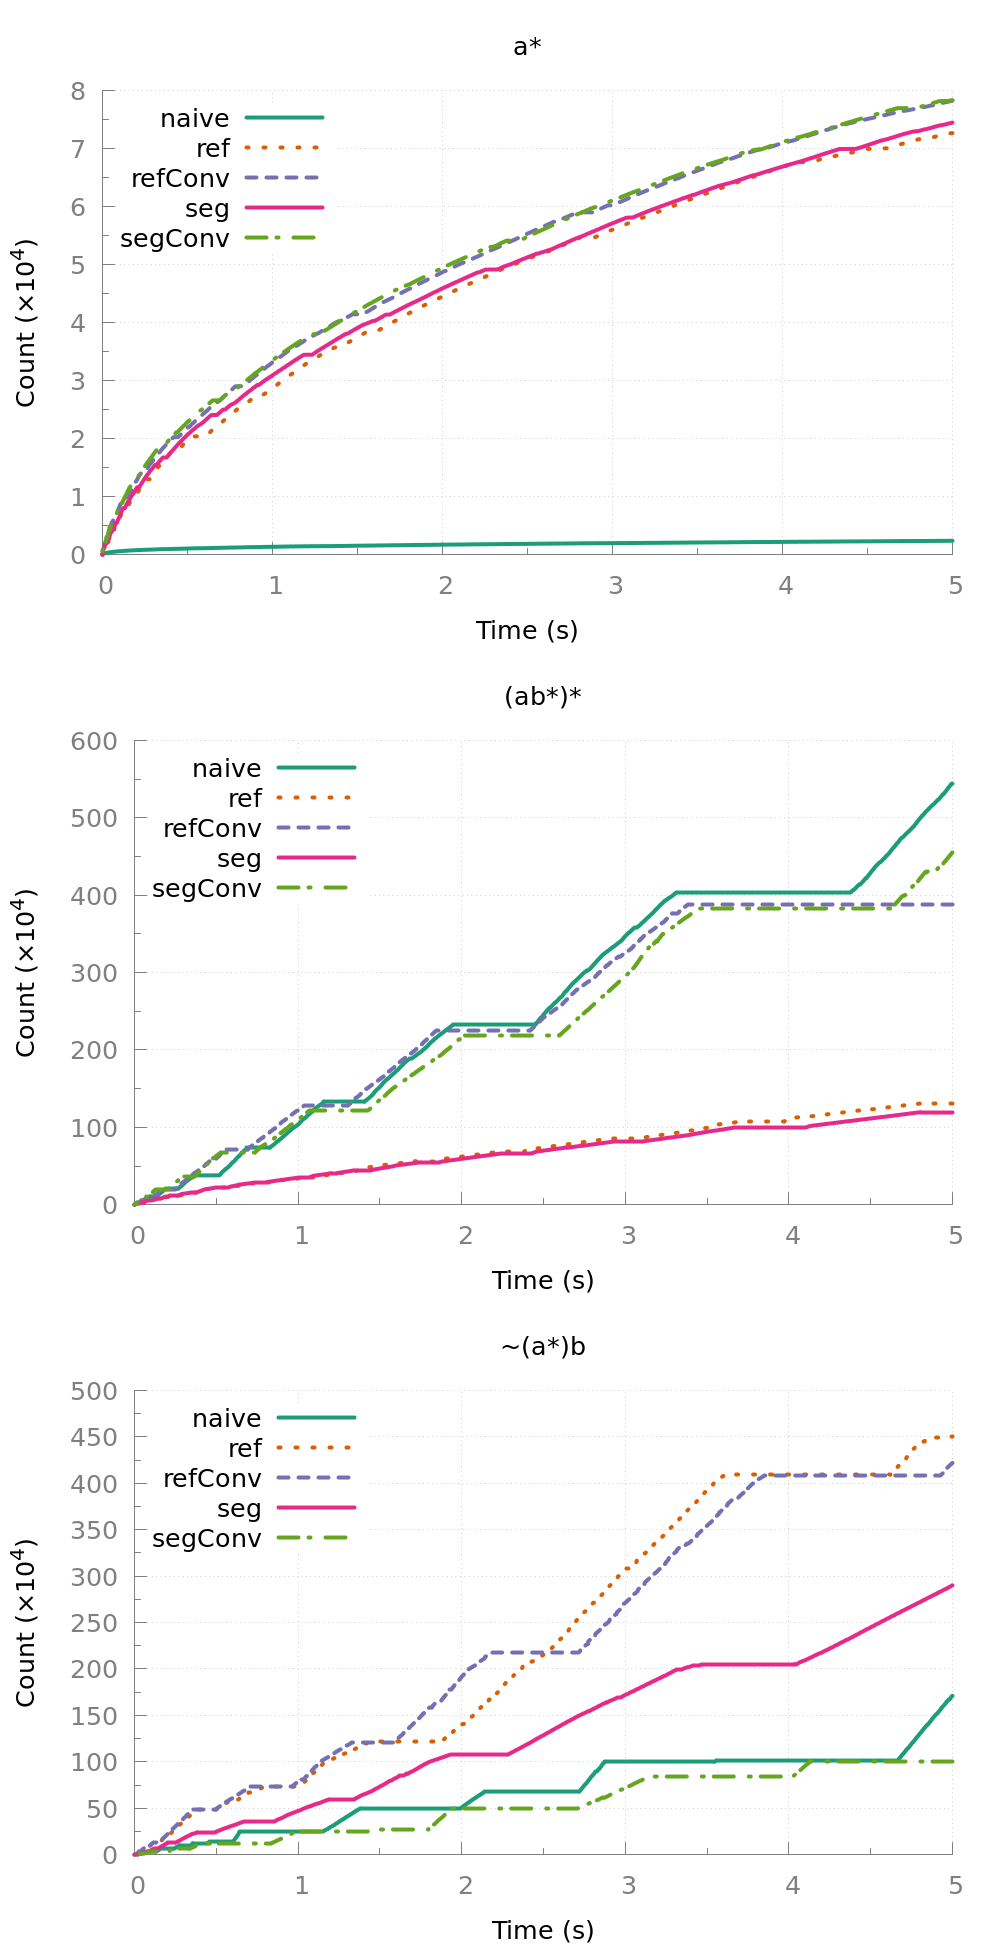
\includegraphics[width=\linewidth]{measure/haskell_all.png}
  \caption{Benchmark for the \haskell implementation with various algorithms}
  \label{bench:haskell:all}
\end{figure}

\subsection{Comparing data-structures in the \ocaml implementation}

We followed the same benchmarking methodology than for the \haskell
version in \autoref{sec:bench}. Benchmark for various data-structures
for regular expressions \verb/a*/, \verb/(ab*)*/ and \verb/~(a*)b/ are
presented in \autoref{bench:ocaml:all}.

\begin{figure}[h]
  \centering
  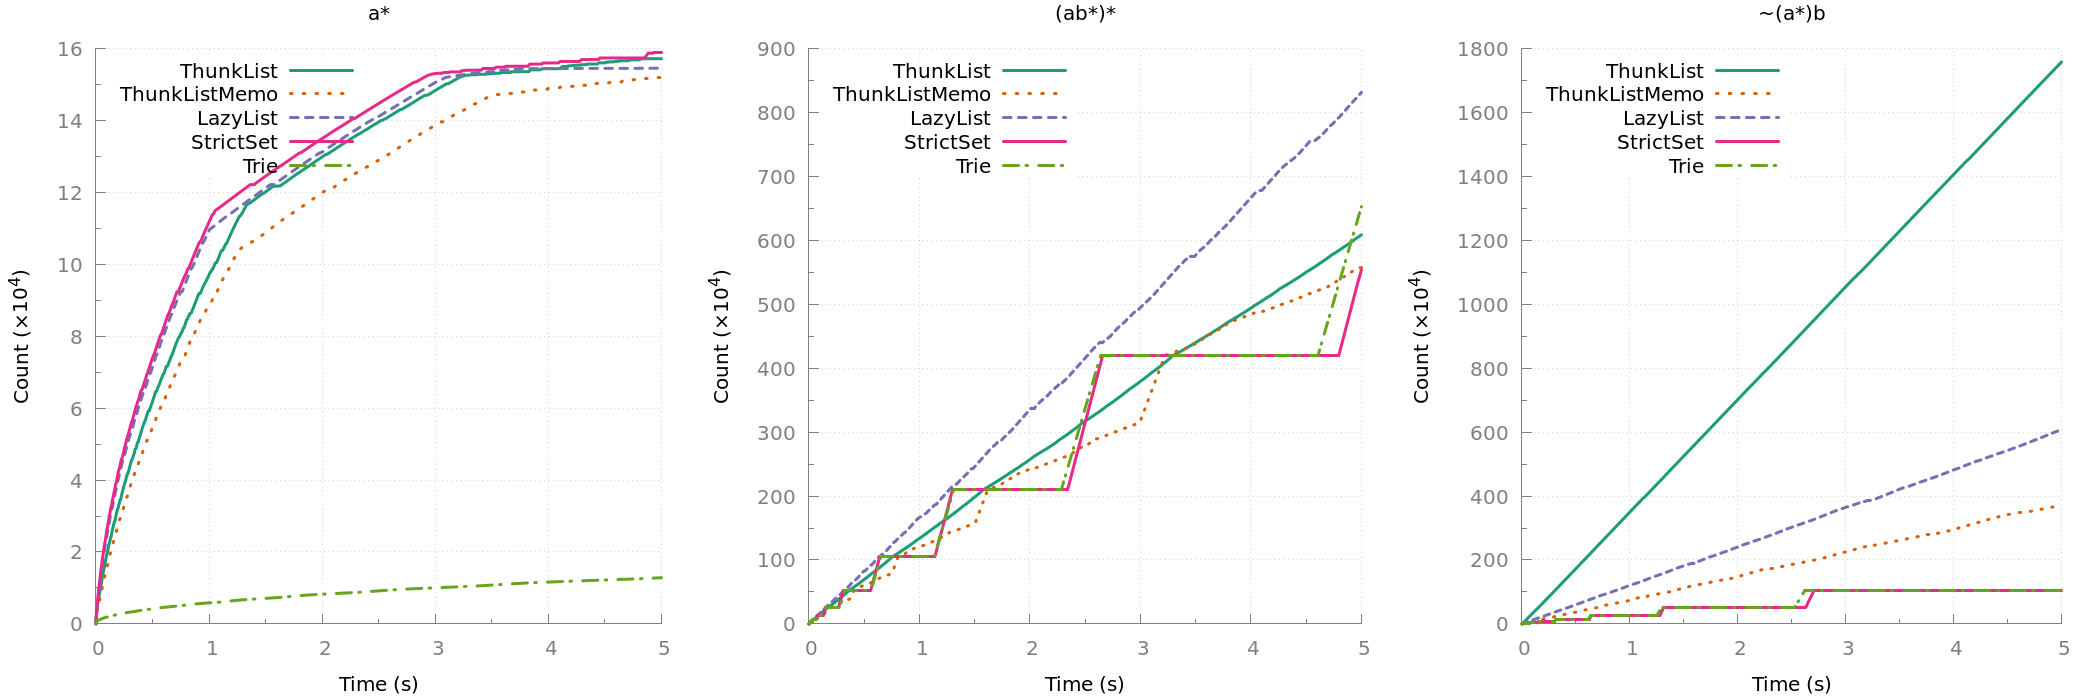
\includegraphics[width=\linewidth]{measure/ocaml_all.png}
  \caption{Benchmark for the \ocaml implementation with various data-structures}
  \label{bench:ocaml:all}
\end{figure}

\subsection{The influence of regular expressions on performances}


\begin{figure}[h]
  \centering
  \begin{subfigure}{0.5\linewidth}
    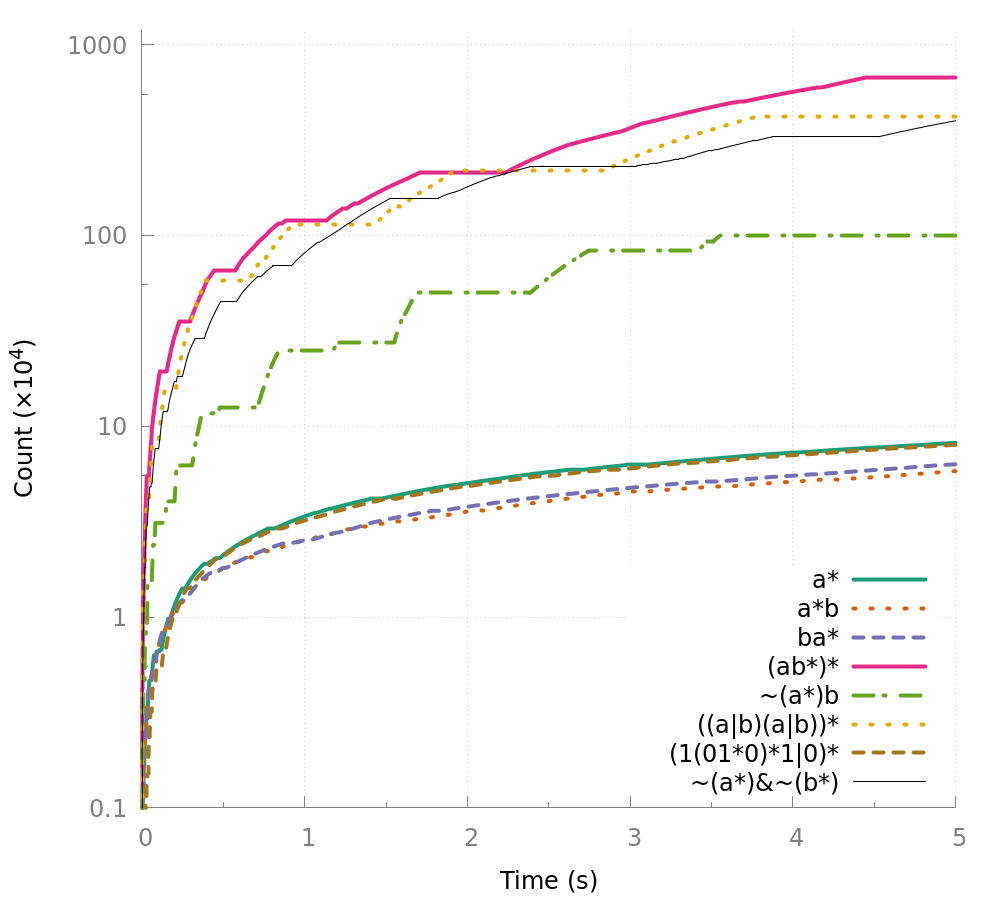
\includegraphics[width=\linewidth]{measure/haskell_langs.png}
    \caption{\haskell implementation with \code{segConv}}
    \label{bench:haskell:langs}
  \end{subfigure}~
  \begin{subfigure}{0.5\linewidth}
    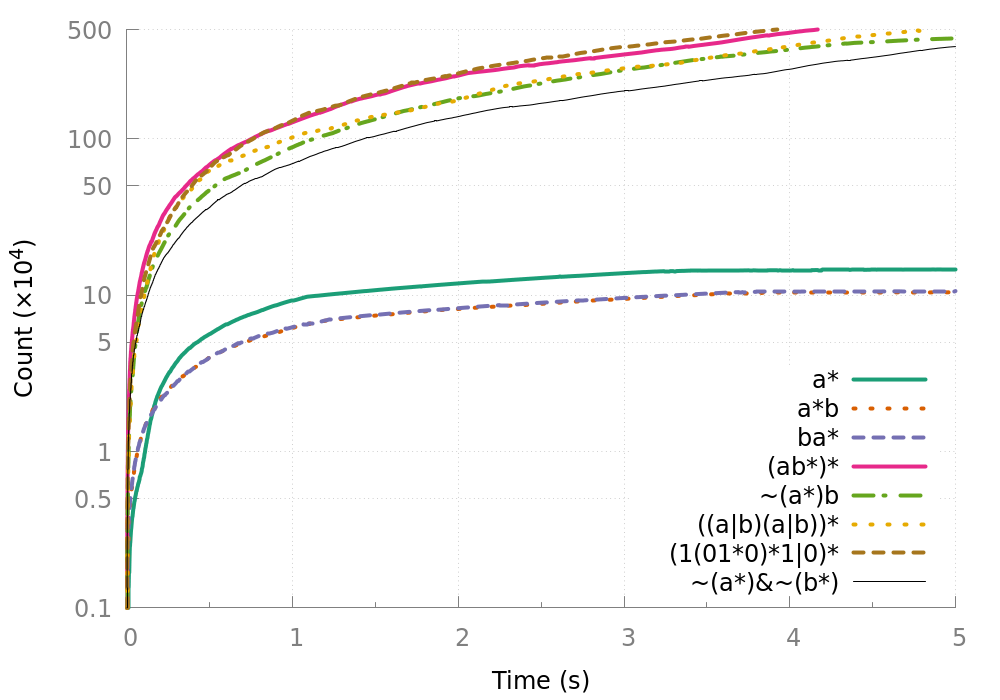
\includegraphics[width=\linewidth]{measure/ocaml_langs.png}
    \caption{\ocaml implementation with \code{ThunkList}}
    \label{bench:ocaml:langs}
  \end{subfigure}
  \caption{Benchmark on different regular expressions}
  \label{bench:langs}
\end{figure}

%%% Local Variables:
%%% mode: latex
%%% TeX-master: "main"
%%% End:

\section{Related Work}
\label{sec:related-work}

\subsubsection*{Regular Language Generation}

\citet{DBLP:journals/actaC/Makinen97} describes a method to enumerate
the words of a regular language $L$ in length-lexicographic
ordering. It relies on the regular language being defined by a
deterministic finite automaton. To generate words up to length $n$,
this method requires to precompute, for each $i\le n$, the
lexicographically minimal and maximal word of length $i$ in $L$. This
precomputation takes time $O(n)$.

The actual enumeration starts with the precomputed minimal word of
length $n$ and repeatedly computes the lexicographically next word
until it reaches the maximal word of length $n$. Each such step requires time $O(n)$. 

The same approach can be used for enumerating the language of certain
(prefix-free, length complete) context-free grammars, too.

Compared to our approach, M{\"{a}}kinen requires a deterministic
finite automaton, which can be obtained from a regular expression in
worst-case exponential time. Complementation is not mentioned, but it
can obviously be handled. M{\"{a}}kinen would give rise to a
productive definition by segments because the computation of minimal
and maximal words could be done incrementally, but which is not mentioned
in the paper.

\citet{DBLP:journals/jfp/McIlroy04} implements the enumeration of all
strings of a regular language in Haskell. He develops two approaches,
one based on interpreting regular expressions, the other (unrelated to
ours) using a shallow embedding of nondeterministic finite
automata. The first approach is inspired by an earlier note by Misra
\cite{misra11:_enumer_strin_regul_expres} and uses operators based on
a length-lexicographically increasing list representation similar to
our first proposal.

The implementation of union is identical to ours, but intersection and
difference operations are not considered and hence complementation is
not considered, either. The implementation of concatenation is the
generic multiplication operation for sequences / power series
\cite{DBLP:journals/jfp/McIlroy99} instantiated for the semiring
of union and concatenation of languages. Unlike our implementation, the generic 
implementation does not take advantage of the fact that many
intermediate results can be generated in the correct ordering and hence
requires many more union operations (one for each output string versus
one for each length between $0$ and $n$ where $n$ is the length of
the output string).  Moreover, the generation method is reported to
be very inefficient and thus not suitable for generating test inputs
at a large scale.

\citet{DBLP:conf/wia/LeeS04} discuss enumerating regular expressions
and their languages. Despite the title, this work is unrelated
because it aims to find bounds on the number of languages that can be
represented with regular expressions and automata of a certain size.

\citet{DBLP:journals/tcs/AckermanS09} improve on M{\"{a}}kinen's
algorithm by working directly on a nondeterministic finite automaton
and by proposing more efficient algorithms to compute minimal words of
a given length and to proceed to the next word of same length in the
language. An empirical study compares a number of variations of the
enumeration algorithm.

Their enumeration algorithm iteratively invokes a cross-section
enumeration, where the $n^{\text{th}}$ cross-section of a language $L$ is
$L \cap \Sigma^n$, that is, a segment in our terminology.

Compared to our work, Ackerman's approach does not incur an
exponential blowup when converting from a regular expression. As it is based on
nondeterministic finite automata, complementation cannot readily be
supported. Moreover, the approach is not compositional.

% They critize his complexity analysis, which assumes unit
% cost for comparison and concatenation operations on words and does not
% account for the size $s$ of the automaton, and obtain $O (s^2n^2)$ for
% the computation of minimal words.


\subsubsection*{Language Generation}
Some authors discuss the generation of test sentences from grammars for
exercising compilers
(e.g., \cite{DBLP:conf/cisse/ParachaF08,DBLP:conf/compsac/ZhengW09}
for some recent work). This
line of work goes back to Purdom's sentence generator for testing
parsers \cite{purdom72:_senten_gener_testin_parser}, which creates
sentences from a context-free grammar using each production at least
once.

Compared to our generator, the previous work starts from context-free
languages and aims at testing the apparatus behind the parser,
rather than the parser itself. Hence, it focuses on generating
positive examples, whereas we are also interested in counterexamples.

Grammar Testing~\cite{DBLP:conf/fase/Lammel01} aims to
identify and correct errors in a grammar by exercising it on example
sentences. The purpose is to recover ``lost'' grammars of programming
languages effectively.
Other work \cite{DBLP:conf/compsac/LiJLG04} also targets
testing the grammar, rather than the parser.

\subsubsection*{Test Data Generation}

Since the introduction of
QuickCheck~\cite{DBLP:conf/icfp/ClaessenH00}, property testing and
test-data generation has been used successfully in a wide variety of
contexts.  In property testing, input data for the function to test is
described via a set of combinators while the actual generation is
driven by a pseudo-random number generator. One difficulty of this
approach is to find the correct distribution of inputs that will
generate challenging test cases. This problem already arises with
recursive data types, but it is even more pronounced when generating
test inputs for regular expressions because, as explained in
\cref{sec:motivation}, many languages have a density of zero, which
means that a randomly generated word almost never belongs to the
langer.  Generating random \emph{regular expressions} is much
easier. We can thus combine property testing to generate regular
expressions and then apply our language generator to generate targeted
positive and negative input for these randomly generated regular
expressions.

\citet{DBLP:journals/jfp/NewFFM17} are concerned with the enumeration
of elements of various data structures. Their approach is
complementary to test-data generators. They exploit bijections between
natural numbers and the data domain and develop a quality criterion
for data generators based on a notion of fairness. It would be
interesting to investigate the connection between their enumeration
strategies and a direct representation of formal power series.

Crowbar~\cite{crowbar} is a library that combines property testing
with fuzzing.  In QuickCheck, the generation is driven by a random
number generator. Crowbar replaces this generator by
\texttt{afl-fuzz}~\cite{afl}. Afl is a fuzzer that relies on runtime
instrumentation to provide good code coverage, thus eliminating the
need to specify the distribution of random generators.  This approach,
however, is not sufficient to generate both regular expressions and
inputs, as we would still require an oracle. Our language generator
could allow to easily fuzz regular expression parsers.


% \subsubsection*{Testing Program Generators}

%%% Local Variables:
%%% mode: latex
%%% TeX-master: "main"
%%% End:

\section{Conclusions and Future Work}
\label{sec:conclusions}


In \cref{sec:bench}, we saw that the performance of our generator highly depends
both on the shape of the language and the shape of the regular expression.
We noticed a rough correlation with the size of each segments, but did not
provide a more precise account. One might wonder if such an account is possible
and if yes, can we use this information to improve language generation
(by transforming a regular expression to an equivalent yet more efficient one).


Generalize to words with weights by replacing boolean with another semiring.

Generate CFLs in this way?

Any decidable language can be enumerated in this way!

Faithful representation as a formal power series: stream of coefficients from a semiring.

Amenable to formalization in Agda?

%%% Local Variables:
%%% mode: latex
%%% TeX-master: "main"
%%% End:


%% Acknowledgments
% \begin{acks}
% \end{acks}

\clearpage
\bibliography{biblio}

% \appendix
% \normalsize

\end{document}
%%% Local Variables:
%%% mode: latex
%%% TeX-master: t
%%% End:
